\section{Zeit- und Frequenzbereich}
Bisher haben wir Signale (sowohl stetige als auch diskrete) ausschließlich im sog. 
\textit{Zeitbereich} betrachtet. Hier tritt unser Signal in Form einer Welle in Erscheinung.
Diese Darstellung ist aber hinsichtlich der darin enthaltenen Frequenzen wenig aufschlussreich.
Anders ist es mit dem \textit{Frequenzbereich} desselben Signals, was die folgende Grafik veranschaulicht:

\begin{figure}[htbp]
    \centering
    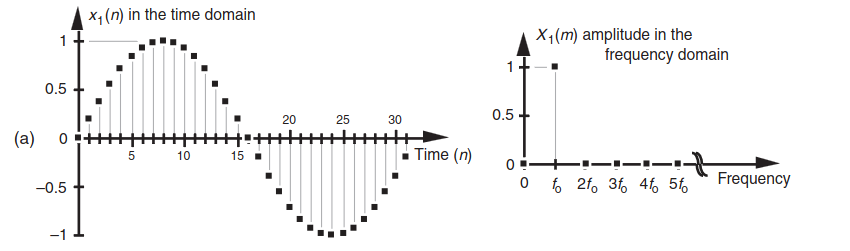
\includegraphics[width=0.8\textwidth]{graphic/img/chapter2/Lyons_time_freq_domain.png}
    \caption{Links: Zeitbereich eines Signals, Rechts: Frequenzbereich desselben Signals \cite[Kap. 1, S. 6]{lyons2010}}
    \label{fig:time_freq_domain}
\end{figure}

Wie in Abbildung \ref{fig:time_freq_domain} illustriert, beschreibt der Zeitbereich eines Signals (links)
mit seiner horizontalen Achse die voranschreitende Zeit in $n$ (\textit{Samples}) und
mit seiner vertikalen Achse die Momentanamplituden zum jew. Zeitpunkt einer Abtastung.

Der Frequenzbereich hingegen zeigt das komplette Spektrum an Frequenzen, die das Signal beinhaltet.
Man kann sich den Frequenzbereich wie ein Prisma vorstellen, das einfallendes, weißes Licht klar sichtbar in seine farbigen spektralen
Bestandteile zerlegt.
Hier steht die vertikale Achse für die jeweilige Frequenzstärke, als positiver Amplitudenwert definiert.
Die horizontale Achse repräsentiert die Frequenz in $Hz$ (bei Audiosignalen wären das verschiedene Tonhöhen, die
gleichzeitig und in verschiedenen Stärken erklingen). \cite[Kap. 2]{lyons2010}
